\section{Results}
\label{sec:results}
% Mention stop agents

The results were collected by training and validating the agent against three opponents at the same time of the same type. During training and validation primarily two types of agents were used, namely the random and simple agents from the Pommerman environment used. Occasionally was our stop agent used as well.

The first model that was trained was utilising the REINFORCE algorithm, see section~\ref{sec:reinforce}, our convolutional network, see section~\ref{sec:conv}, the $\epsilon$-greedy strategy with decay, see figure~\ref{fig:gamma}(a), a static board, see section~\ref{sec:static}, and finally the standard reward function of $-1$ for a loss and $1$ for a win. In figure~\ref{fig:resultsrandom} the validation and training error of the agent trained against three random agents is displayed. Remember that with the $\gamma$ function used for the $\epsilon$-greedy strategy the agent will keep exploring until approximately $85\%$ of the iterations has been played. From figure~\ref{fig:resultsrandom} one can see that around the $85\%$ mark the validation and training rewards are both $1.00$, but already from the first validation is the agent achieving a reward of $1$. Looking at the actions the agent were performing, it is clear to see that the agents has learning to perform any single action that is not placing a bomb, thereby waiting for the random agents to kill themselves and winning the game.

\begin{figure}[htb]
    \centerline{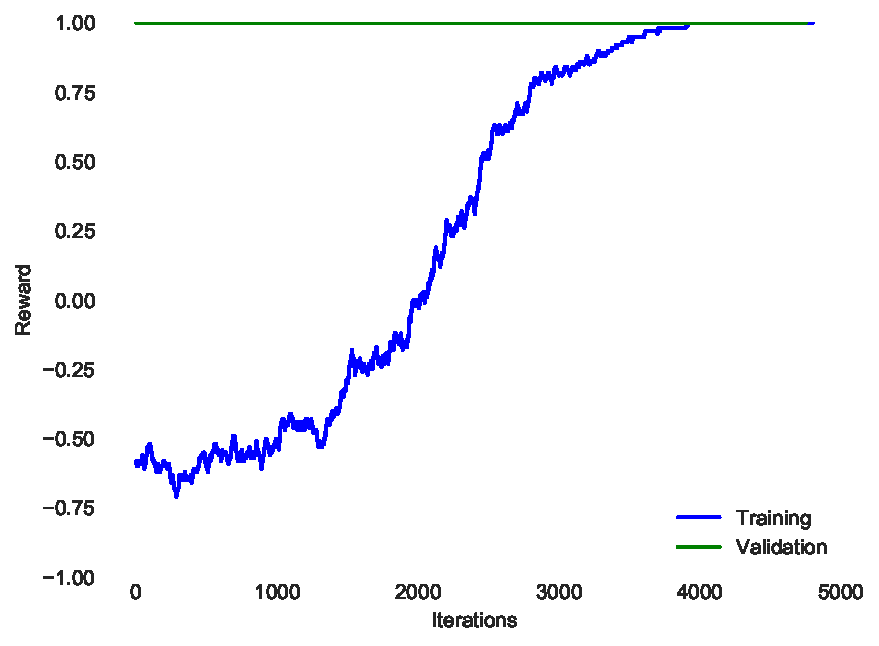
\includegraphics[width=1.0\linewidth]{pommerman/plots/random_train_val.pdf}}
    \caption{Moving average of validation and training rewards against random agents.}\label{fig:resultsrandom}
\end{figure}

In figure~\ref{fig:resultssimple} the validation and training rewards of the agent trained against three simple agents are displayed, using the same model as against the three random agents. From figure~\ref{fig:resultssimple} it is seen that there is a slight incline in the training reward as the agent starts to exploit more and more. However, it does seem to flatten a bit towards the last 5000 iterations. The incline is due to the simple agents are killing each other and themselves without our agent killing itself, thereby never reaching our agent and leaving it to win and receive a reward of $1$. Looking at the reward for the validation it seems to be moving around an average of $-0.65$, with a slight incline in the reward towards the end of the training of the agent.

\begin{figure}[htb]
    \centerline{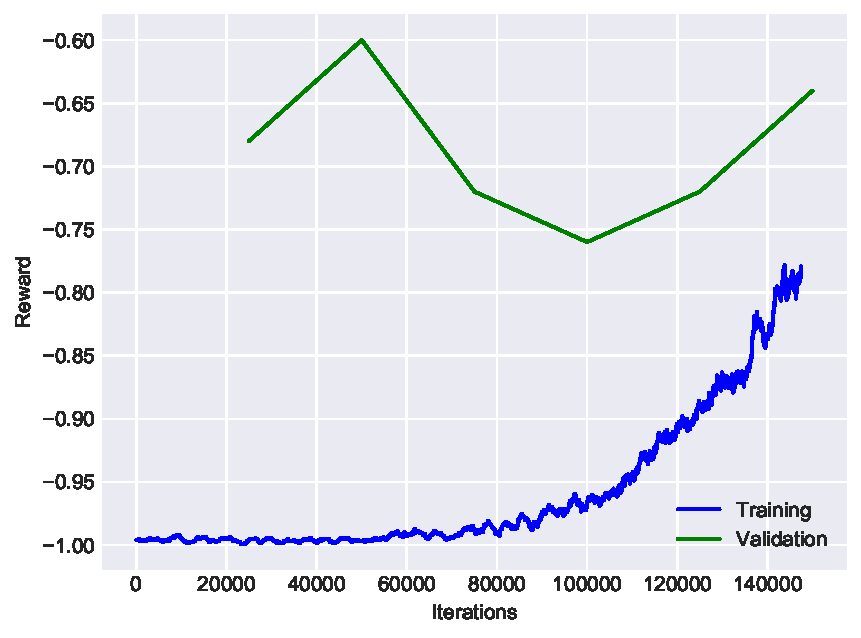
\includegraphics[width=1.0\linewidth]{pommerman/plots/train_val.pdf}}
    \caption{Moving average of validation and training rewards against simple agents.}\label{fig:resultssimple}
\end{figure}

The probabilities of each action during the training against the three simple agents can be seen in figure~\ref{fig:act}. From this it is evident that the probability of the two actions \emph{Down} and \emph{Right} are in a constant incline, the probability for \emph{Bomb} is on a constant decline and the remaining actions are fairly stable until the \nth{105000} iteration. After that the probability of the action \emph{Down} increases extremely fast towards $1$ and the remaining probabilities decreases towards $0$. Now that it is clear that the agent is performing a single action towards the end of where it fully exploits, the incline in its training and validation rewards is purely because of the actions of the other agents. Had the agent been run for more iterations where it would fully exploit, it would most likely be the case that the two rewards would go towards each other and be stationary around the same reward.

\begin{figure}[htb]
    \centerline{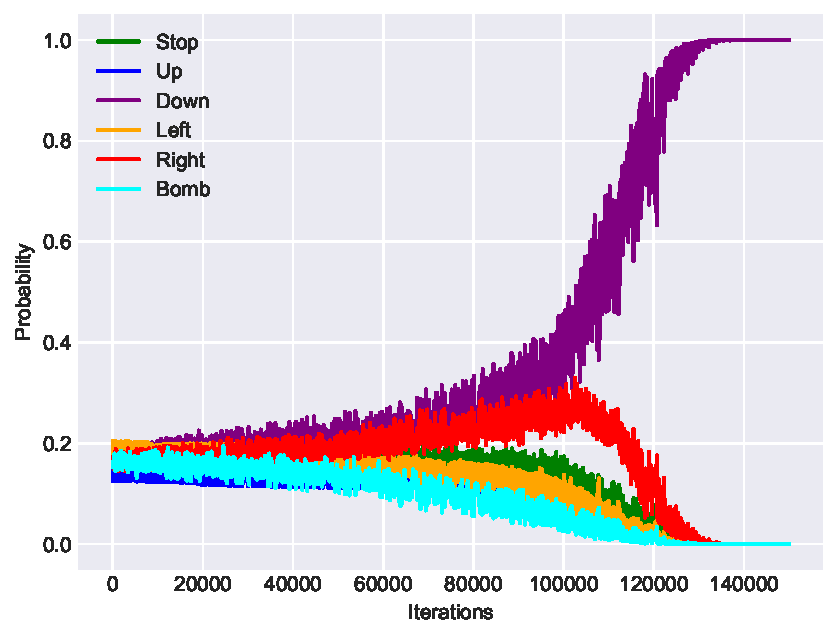
\includegraphics[width=1.0\linewidth]{pommerman/plots/a_probs.pdf}}
    \caption{Distribution of action probabilities.}\label{fig:act}
\end{figure}

% THIS HAS TO BE ADJUSTED IF WE ADD THE RESULT OF THE MODEL USING THE CUSTOM REWARD FUNCTION.
It should be emphasised that despite only showing the results of one model, the agent has been trained with numerous different models. The models have had its hyper parameters changes, different networks and sizes and reward functions. Furthermore have they been trained against the standard dynamic boards and our custom static board. Each configuration has been run for $150.000$ games. However, despite these different configurations all networks ended up producing the near same rewards results and converged towards picking one action, as was the case shown in figure~\ref{fig:act}. This also turned out to be independent of whether REINFORCE or Q-learning was used.

% Sometimes mentioned as experiments/results. Maybe experiments sounds better for us xD
% Show that the agent was able to learn playing against 3 random agents
% Show graphs for result for playing against 3 simple agents (-1 constantly, easy graph)

%\subsection{Performance}
% As in iterations, training time etc.
% Mention the number of iterations 

% Result for every method used should be stated